\documentclass[12pt,a4paper,oneside]{article}
\special{papersize=8.5in,11in}

\setlength{\textwidth}{6.5in} %1 in margins
\setlength{\textheight}{9.75in}
\setlength{\oddsidemargin}{0in}
\setlength{\topmargin}{0in}
\setlength{\headheight}{0in}
\setlength{\headsep}{0in}
\setlength{\marginparwidth}{1in}
\setlength{\footskip}{0.25in}
\setlength{\marginparsep}{0in}

\renewcommand{\abstractname}{}

\usepackage{amssymb,amsmath}
\usepackage{multirow}
\usepackage{subfigure}
\usepackage{graphicx}
\usepackage{graphics}

\usepackage{caption}
\usepackage{color}
\usepackage{listings}
\usepackage{courier}
\lstset{
  basicstyle=\footnotesize\ttfamily, % Standardschrift
    %numbers=left,               % Ort der Zeilennummern
    numberstyle=\tiny,          % Stil der Zeilennummern
    %stepnumber=2,               % Abstand zwischen den Zeilennummern
    numbersep=5pt,              % Abstand der Nummern zum Text
    tabsize=2,                  % Groesse von Tabs
    extendedchars=true,         %
    breaklines=true,            % Zeilen werden Umgebrochen
    keywordstyle=\color{red},
    frame=b,         
    %        keywordstyle=[1]\textbf,    % Stil der Keywords
      %        keywordstyle=[2]\textbf,    %
      %        keywordstyle=[3]\textbf,    %
      %        keywordstyle=[4]\textbf,   \sqrt{\sqrt{}} %
      stringstyle=\color{white}\ttfamily, % Farbe der String
      showspaces=false,           % Leerzeichen anzeigen ?
      showtabs=false,             % Tabs anzeigen ?
      xleftmargin=17pt,
    framexleftmargin=17pt,
    framexrightmargin=5pt,
    framexbottommargin=4pt,
    %backgroundcolor=\color{lightgray},
    showstringspaces=false      % Leerzeichen in Strings anzeigen ?        
}
\lstloadlanguages{% Check Dokumentation for further languages ...
  %[Visual]Basic
    %Pascal
    %C
    C++
    %XML
    %HTML
    %Java
}
%\DeclareCaptionFont{blue}{\color{blue}} 

%\captionsetup[lstlisting]{singlelinecheck=false, labelfont={blue}, textfont={blue}}
\usepackage{caption}
\DeclareCaptionFont{white}{\color{white}}
\DeclareCaptionFormat{listing}{\colorbox[cmyk]{0.43, 0.35, 0.35,0.01}{\parbox{\textwidth}{\hspace{15pt}#1#2#3}}}
\captionsetup[lstlisting]{format=listing,labelfont=white,textfont=white, singlelinecheck=false, margin=0pt, font={bf,footnotesize}}


\begin{document}

\author{Joshua Gleason}
\title{CS 476 Programming Assignment 1}
\date{September 9, 2010}

\maketitle

\begin{abstract}
{ \bf
  In this project I wrote two simple image processing programs.  The first is designed
  to change the spacial resolution of a 256 x 256 image to 128 x 128, 64 x 64, and 32 x 32.
  It then needs to resize the image for viewing purposes to determine how much quality was
  lost in the spacial reduction.  The other program performs quantization on an image,
  changing the number of bits per pixel from 8 to 6, 4, and 2.  In other words, the number
  colors in the image is reduced from 256 to 64, 16, and 4.
}
\end{abstract}

\section{Method}
  The reduction of an images spacial resolution can be done using a number of methods.
  The method I choose to use was to average the pixels in the area which was to be
  sampled down, then use that average as the pixel value in the reduced image.  I choose
  this method over simply sampling, because much more information is retained, and this
  also helps reduce the amount of noise in the image.

  For the second program, I wanted to quantize the image, so first I had to sample the
  develop an intensity transformation function which would map the original 256 colors into
  a smaller domain.  Knowing that \( [0,255] \rightarrow [0,f_{max}] \) where $f_{max}$ is
  the maximum value in the new domain; we are able to solve for a linear intensity
  transformation $y=ax+b$ by solving the following system.
  \[
    \begin{split}
    0 & = a(0) + b \\
    f_{max} & = a(255) + b
    \end{split}
  \]

  Solving for $a$ and $b$

  \[
    \begin{split}
    a & = \cfrac{f_{max}}{255} \\
    b & = 0
    \end{split}
  \]

\section{Implementation}
  I choose to implement this program using the OpenCV library.  I choose to do this because
  it saved time, and I didn't see any reason why I should risk building a new Image class
  which could potentially introduce bugs, when a very well build library already exists.
  
  For the first program, rather than simple shrink the image, and then enlarge it again, I
  decided to improve the algorithm by calculating everything without actually shrinking the
  image.  To do this I first calculated the size of the area in the original image which
  would be mapped to a single pixel.  Next I iterated across each region and calculated the
  average, then on the new image filled that region in with the average value.  This method
  is slightly faster than shrinking the image, then enlarging it because it does not require
  the extra memory allocation for the smaller image.

  For the second program, I mapped each pixel into the new domain (where $f_{max} = 3, 15,
  \textup{ or } 63$).  I was able to do this by dividing the current value by
  $\cfrac{256}{f_{max}+1}$. Dividing by $a^{-1}$ is used here to make up for integer
  truncation errors and to remove the need for floating point calculations.  After this step
  the image was normalized back to $[0,255]$ for viewing purposes.

\section{Results}
  For the first program, it is obvious when the dimensionality is reduced to 32 x 32
  and 64 x 64.  It is much harder to tell that the 128 x 128 image has been reduced by
  half.  This is a rather interesting results, as it shows that even with a substantial
  loss in memory, for many purposes lower resolution images may be worthwhile.  Images
  tend to take up a lot of space in a computer, reducing the resolution by half, reduces
  the size of the image to a quarter of it's original, and it does it without losing a great
  deal of quality.

  The second program, it is also obvious that the depth of the image has been reduced in the
  2 bit and 4 bit images, but with the 6 bit image it is identical to the original according
  to my eyes.  This brings up another interesting observation.  It it possible to reduce the
  depth of the image to 3 quarters of its original without any visible loss of quality.  This
  quality could also be used to reduce to size of the images.  In fact if we were to reduce
  the size of an image by half, and reduce its depth to 6 bits, the size of the image would
  reduce to three sixteenths of its original size.

\pagebreak

\section{Source Code}
  \lstinputlisting[caption=resample.cc]{resample.cc}
  \lstinputlisting[caption=quantize.cc]{quantize.cc}
  \lstinputlisting[caption=generic.h]{generic.h}

\pagebreak

\section{Images}

\begin{figure}[hbt]
  \centering
  \subfigure[Original]{
    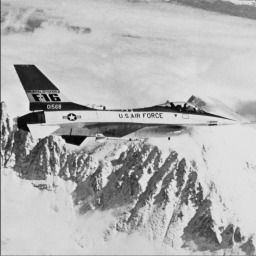
\includegraphics[width=128pt]{f_16}
  }
  \subfigure[{\scriptsize 128x128 at 4 $\cfrac{\textup{bit}}{\textup{pix}}$ \scriptsize (12.5\% mem)}]{
    \includegraphics[width=128pt]{f_16_128_4bit} 
  }
  \subfigure[{\scriptsize 128x128 at 6 $\cfrac{\textup{bit}}{\textup{pix}}$ \scriptsize (18.8\% mem)}]{
    \includegraphics[width=128pt]{f_16_128_6bit}
  } \\
  \subfigure[128x128]{
    \includegraphics[width=128pt]{f_16_128}
  }
  \subfigure[64x64]{
    \includegraphics[width=128pt]{f_16_64}
  }
  \subfigure[32x32]{
    \includegraphics[width=128pt]{f_16_32}
  } \\
  \subfigure[6 bit/pix]{
    \includegraphics[width=128pt]{f_16_6bit}
  }
  \subfigure[4 bit/pix]{
    \includegraphics[width=128pt]{f_16_4bit}
  }
  \subfigure[2 bit/pix]{
    \includegraphics[width=128pt]{f_16_2bit}
  }
\end{figure}

\begin{figure}
  \centering
  \subfigure[Original]{
    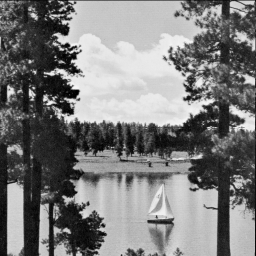
\includegraphics[width=128pt]{boat} 
  }
  \subfigure[{\scriptsize 128x128 at 4 $\cfrac{\textup{bit}}{\textup{pix}}$ \scriptsize (12.5\% mem)}]{
    \includegraphics[width=128pt]{boat_128_4bit} 
  }
  \subfigure[{\scriptsize 128x128 at 6 $\cfrac{\textup{bit}}{\textup{pix}}$ \scriptsize (18.8\% mem)}]{
    \includegraphics[width=128pt]{boat_128_6bit} 
  } \\

  \subfigure[128x128]{
    \includegraphics[width=128pt]{boat_128}
  }
  \subfigure[64x64]{
    \includegraphics[width=128pt]{boat_64}
  }
  \subfigure[32x32]{
    \includegraphics[width=128pt]{boat_32}
  } \\

  \subfigure[6 bit/pix]{
    \includegraphics[width=128pt]{boat_6bit}
  }
  \subfigure[4 bit/pix]{
    \includegraphics[width=128pt]{boat_4bit}
  }
  \subfigure[2 bit/pix]{
    \includegraphics[width=128pt]{boat_2bit}
  }
\end{figure}
\end{document}

